\documentclass[12pt,a4paper]{article}
\usepackage{graphicx}
\usepackage{amsmath}
\usepackage{float}
\graphicspath{ {../Result/} }

\title{Model fitting for thermal responses of metabolic traits}
\author{Student:Shiyun Liu\\ s.liu18@imperial.ac.uk}
\date{ }

\begin{document}
\maketitle

\newpage

\section{Abstract}
For many years, global warming has been and is still a trending topic in both public and academic field. This long-term increase of temperature in worldwide has been witnessed as a pronounced representation of global climate change. The effects of global warming influence not only human society but also directly act on ecosystem and have a huge impact on other living organisms. One of the studying fields that focuses on temperature changes and species population is the thermal responses of metabolic traits. Since model fitting has always been a good approach to study relationships in biology. To find out how metabolic traits react to changing temperature, we can fit mathematical models to the observed data and predict the relationship. In this study, I am trying to fit 5 different models to thermal responses of metabolic traits using computational analysis and find the more appropriate model via model comparison.

\section{Introduction}
\subsection{Global warming}
Global warming is an aspect of global climate change featured by the rise in the average temperature during decades in terms of the the whole Earth. It is commonly referred to the predominantly human-caused temperature rise after pre-industrial times. The major influence caused by human is the great amount of greenhouse gases emission, which includes carbon dioxide, methane, and nitrous oxide. The effects of global warming include but not limited to aspects such as environmental changes (sea level rise, ocean acidification, extreme weather,  deserts expansion and ecosystem changes), social impacts (crop production and general impact on public health) and biosphere damages (reduced biodiversi).
\cite{globalwarming}
\subsection{Thermal response of metabolic trait}
One of many aspects that shows rising temperature can be a serious issue is about the growth and development for living creatures on both individual and population levels. In terms of evolution, it is reported that temperature change can affect the rate of evolution and the mutation rate may rise in warmer environment. 
\cite{evolution}
In terms of ecology, the temperature increase could lend to different metabolic levels. And the metabolic rate can directly influence the intrinsic rate of exponential population growth and the carrying capacity. 
\cite{ecology}
Therefore thermal responses of metabolic rate can have an impact on population dynamics. Also the growth and survival for species population and ecosystem stability is seen to be temperature dependent, as the majority of life (99.9\%) on earth is ectothermic and the metabolic reactions of plants is crucial for other organisms in the ecosystem.
\subsection{Mechanistic models and phenomenological models}
There are two types of scientific models using to describe and predict the relationship between data or phenomena. One of them is phenomenological model, which try to build statistically significant, non-random pattern from empirical data. The other one is mechanistic model, which intend to describe the mechanisms underlying the pattern in empirical data. The main difference between the two models is that mechanistic model has a theoretical basis and it is derived from first principle. On the contrast, phenomenological model makes no assumption on the mechanisms behind the pattern and it does not have a theoretical basis. 
In this study, the two phenomenological models are cubic model and Briere model. The cubic model is one type of polynomial models with 4 parameters. They are famous phenomenological models. The mechanistic models used in this study are Schoolfield models including one full model and two simplified versions. This model is a biological temperature dependent rate model formulated by R. M. Schoolfield and his colleagues in 1981. It is based on Sharpe and DeMichele’s model and Hultin’s formulation, however with better parameter interpretations and more achievable initial parameter estimation and reduced corralation between parameter estimators.
\cite{schoolfield}
\subsection{Model comparison}
When there are several candidates models which can be applied to a set of data, quantified measurement should be taken to compare the quality of models. The AIC (Akaike information criterion) is one of the estimators for the relative quality of candidate models. It selects the better model based on the criterion of better fit meanwhile fewer parameters. The formula for calculate AIC is 2k + n Log(RSS/n), where k is the number of parameters, n is the number of observation and RSS the residual sums of squares. In general, smaller AIC indicates a better fitted model.
\cite{modelselection}
\section{Method}
\subsection{Data preparation}
The dataset is provided by My mini project supervisor Dr. Pawar. It is collected over years and cooperated by labs across the world. Thanks to the effort of many researchers, I now have this large dataset that contains information on hundreds of thermal responses for metabolic rate such as growth, respiration and photosynthesis rates in plants and bacteria (both aquatic and terrestrial).
\\
In this specific study I am focusing on the ConTemp column which contains temperature recording in Celsius and OriginalTraitValue which reports the metabolic trait value. The metabolic traits in this datasets includes a variety of measurements (18 in total), such as respiration rate, net photosynthesis, specific growth rate, radial growth rate and individual length growth rate. 
Since the type of metabolic trait is consistent for the same species, the types of traits is not distinguished in this study (but still saved in analysis dataset for future analysis). The dataset is grouped by species ID and entries for the same species are give a unique group ID. In the end, columns for GroupID, FinalID, StandardisedTraitName, OriginalTraitValue and ConTemp (the temperature) are extracted from the mata-data file.
\\
This step is done by Rstudio (v.3.5.2) \cite{Rstudio} with dplyr package \cite{dplyr}.
\subsection{Data clearance}
The analysis dataset is extracted from the original dataset and data clearance is done by removing negative or 0 value in Original Trait Value lane and rows that contain NA value. Since these records could be wrong or meaningless data. The groups of observation which have less than 5 entries are also removed. Because the group with too few variables sets is not valuable in modelling especially when the models contain 3 to 6 parameters. The groups whose recorded temperature values are identical are also removed as the data is not informative for model fitting. The column of converted temperature is also added converting the ConTemp column values from Celsius to Kelvin. To facilitate the initial parameter estimation in Schoolfield model, the logarithm or OriginalTraitValue and 1/kT (k is Boltzmann constant) are calculated as well.
\\
This step is done by Rstudio (v.3.5.2) \cite{Rstudio}.

\subsection{Model selection and Initial parameter choosing}
In this study, the 5 models I am going to fit and compare are mentioned above and listed as follow:
\\
1.Cubic polynomial model, which is a phenomenological model, with the 4 parameters (a, b, c, d) lacking mechanistic interpretation.
\begin{equation}
\mathcal B = a+bT+cT^2+dT^3
\\
\end{equation}
The initial values are all set to zero for parameter a,b,c in all group.
\\
2. Briere model, another phenomenological model with 3 parameters B0 (normalization constant),T0 (minimal feasible temperature to keep trait value above 0), Tm (maximal feasible temperature). Although the parameters are more meaningful than cubic model, there is still no enough mechanistic behind the model.
\begin{equation}
\mathcal B = B_0T(T-T_0)\sqrt{T_m-T}
\\
\end{equation}
The initial values for B0 are set to zero for B0. For Tm, it is the maximal temperature in each group of data. Meanwhile T0 is the minimal temperature.
\\
3. Schoolfield model, which is a mechanistic model with thermodynamics and enzyme kinetics theory basis. \\
\begin{equation}
\mathcal B = \frac{B_0e^{\frac{-E}{k}(\frac{1}{T}-\frac{1}{283.15})}}{1+e^{\frac{E_l}{k}(\frac{1}{T_l}-\frac{1}{T})}+e^{\frac{E_h}{k}(\frac{1}{T_h}-\frac{1}{T})}}
\\
\end{equation}
The full model has 6 parameters, which are B0 (trait value at 283.15 K, represents the value of the growth rate at low temperature and controls the vertical offset of the curve), E (activation energy that controls the rise of the curve till the peak, representing the "normal operating range" for the enzyme), Eh ( de-activation energy of an enzyme during high-temperature, which is responsible for the action of the enzyme at very high temperatures), El (he opposite of Eh, which controls the enzyme behaviour at low temperature), Th (the temperature at which the enzyme is 50\% high temperature deactivated) and Tl (the opposite of Th, the temperature when enzyme is 50\% deactivated at low temperature).
\\
The two simplified versions have 4 parameters. They are tailored for situations when low/high temperature inactivation is weak, or measurements taken at that temperature in not detectable.
\begin{equation}
\mathcal B = \frac{B_0e^{\frac{-E}{k}(\frac{1}{T}-\frac{1}{283.15})}}{1+e^{\frac{E_h}{k}(\frac{1}{T_h}-\frac{1}{T})}}
\\
\end{equation}
\begin{equation}
\mathcal B = \frac{B_0e^{\frac{-E}{k}(\frac{1}{T}-\frac{1}{283.15})}}{1+e^{\frac{E_l}{k}(\frac{1}{T_l}-\frac{1}{T})}}
\\
\end{equation}
The initial values for B0 is allocated by the original trait values which corresponding temperatures are closest to 283.15K in each data groups. For E, the initial values are estimated by calculating the slopes on the right hand side of the log-transformed curves (by plotting each data group and calculate the regression lines from the max trait value corresponding point to the max 1/kT point). The Eh initial values are estimated similar to E but they are the slopes on left hand side. The Th initial values are given by the temperature values who maps to the max trait values in each group. The Tl initial values are given by the min temperature values in each data group.
\\
This step is done by Rstudio (v.3.5.2) \cite{Rstudio} as well.
\subsection{Model fitting}
The models were fitted using least square method via Python \cite{python} module lmfit \cite{lmfit}. The main submodule used is minimise, which is used to find the minimal residual for the model. The try-except function is used to bypass the models that fail to converge and allocate the outputs with NA values. The output for calculated parameters and model AIC are saved to new csv files for all 5 models. The modules numpy \cite{numpy} and pandas \cite{pandas} are also used.
\subsection{Graph plotting}
After obtaining the parameter values for converged models, package ggplot2 \cite{ggplot} in Rstudio \cite{Rstudio} is used to plot the original data sets and lines of the successfully fitted models on to the same graph for each data group. The AIC distribution for all fitted models among all groups is also plotted using ggplot2. And by selecting the minimal AIC value among the successfully fitted models in each group, the general performance of all 5 models among 1935 groups of data can be viewed and analysed.


\section{Result}
\subsection{Data preparation and clearance}
The dataset starts with 25826 entries of observation, 24289 left after adjustment of negative or 0 value of trait value, 24136 after remove NA in ConTemp and 23649 after clearing entries of less than 5 in a group. And finally 23625 left after removing 4 groups that have identical temperature records in each group. There are 1935 groups of different species with their thermal response of metabolic traits end up to be tested for 5 models.
\subsection{Model selection and Initial parameter choosing}
The initial parameter finding for Briere model went through smoothly however in parameter calculation for Schoolfield model, errors occurred. 3 groups (17 entries) of E and El, 161 groups (2060 entries) of Eh value were assigned with NA. The NAs of E, Eh and El are all given the median value calculated from the existed dataset, which are -0.5663, 0.5520 and -0.2832 respectively.
\subsection{Model fitting and plotting}
The fitting for cubic model went through smoothly and all 1935 groups of data converge at this model.
\\
The fitting for Briere model also did relatively well, 1913 out of 1935 groups converge.
\\
The result for full Schoolfield model however converge only in 170 groups, less than 10\% of the total dataset. It is also important to notice that there are 362 groups failed to converge because the data entries in these groups are fewer than 6 (5 entries as the fewer are already removed), giving that the parameters in this model is 6.
\\
The two simplified Schoolfield models on the other hand fitted better to the dataset. The low temperature ignored model gets 840 converged groups and high temperature ignored one gets 530 groups.
\\
The results for 5 model fittings are plotted on to 1935 graphs, with group ID as title, original dataset plotted as red points and candidate models plotted in different colours if the model converges. All graphs are saved in model\textunderscore plot\textunderscore all.pdf file which can be viewed in my GitHub repository. And I have also plot graphs for groups where all model converge, and save in model\textunderscore plot.pdf. I hereby only picked some graphs to display the modelling result.

\begin{figure}[H]
\centering
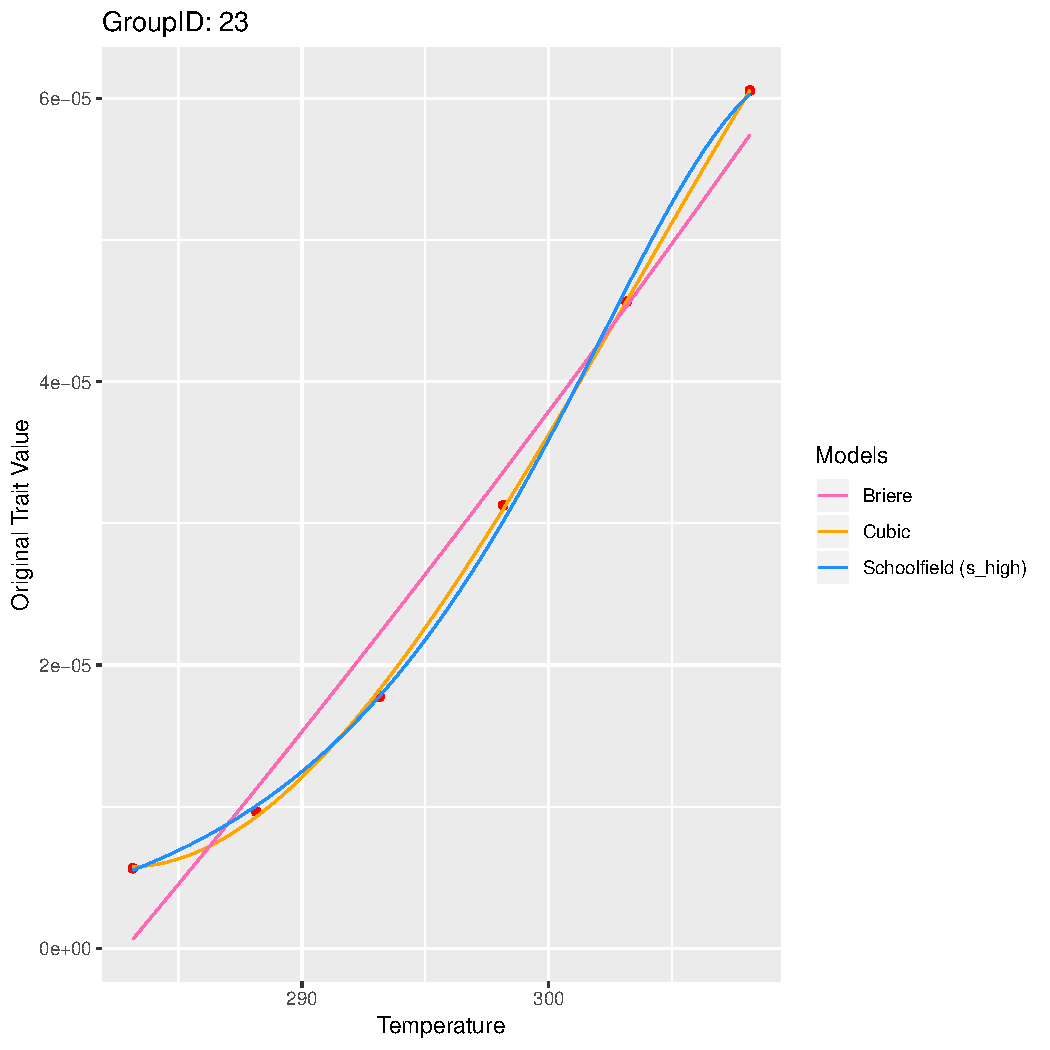
\includegraphics[width=\textwidth]{example1.pdf}
\end{figure}
Figure.1.GroupID 23
\\
\begin{figure}[H]
\centering
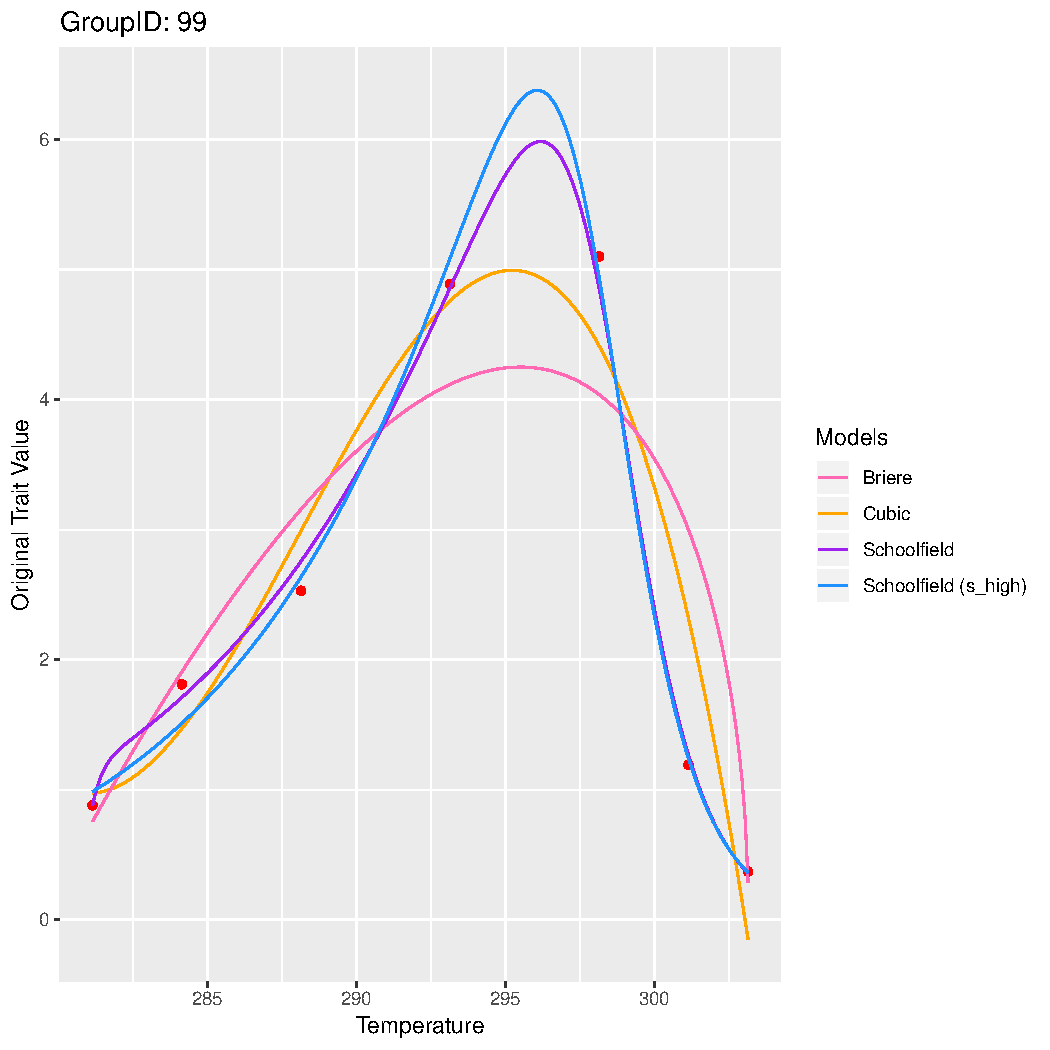
\includegraphics[width=\textwidth]{example2.pdf}
\end{figure}
Figure.2.GroupID 99
\\
\begin{figure}[H]
\centering
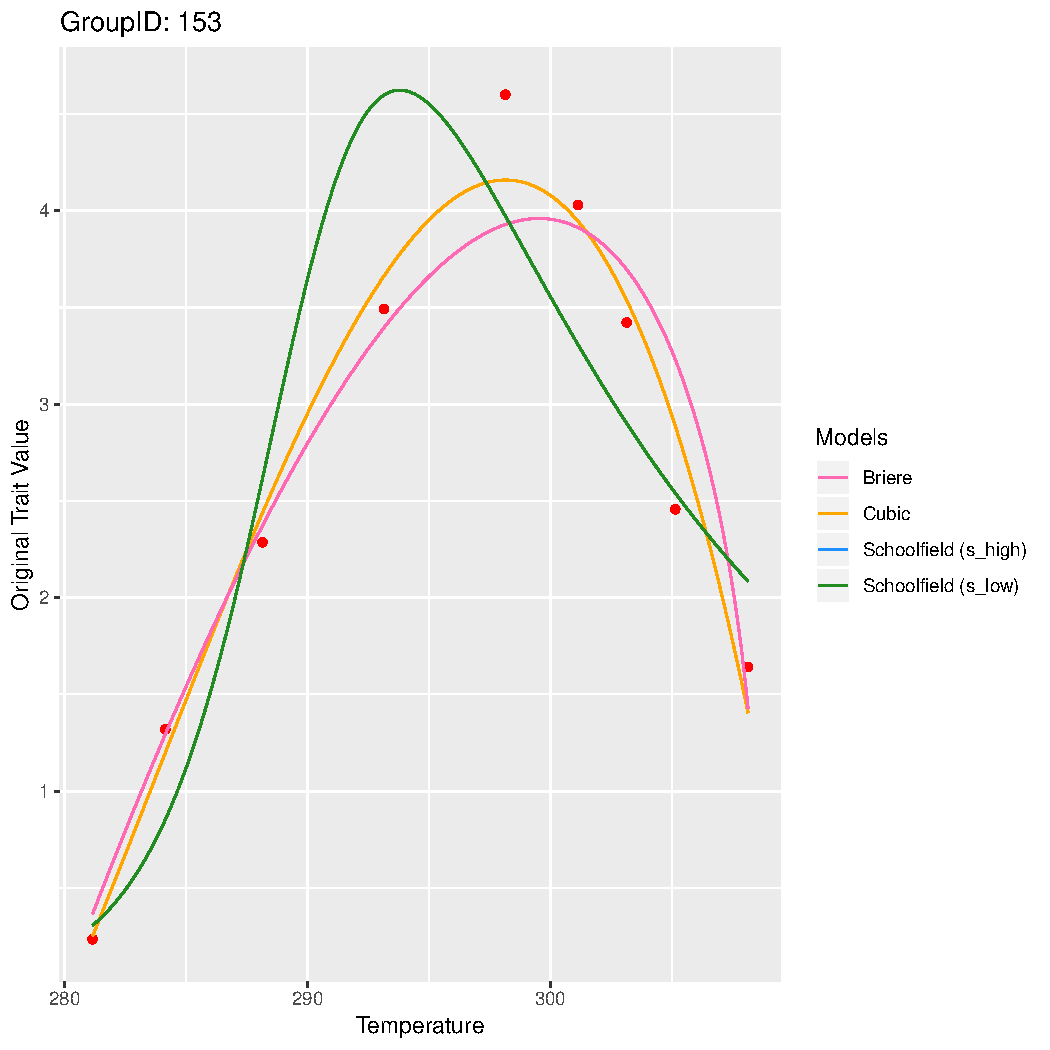
\includegraphics[width=\textwidth]{example3.pdf}
\end{figure}
Figure.3.GroupID 153
\\
\begin{figure}[H]
\centering
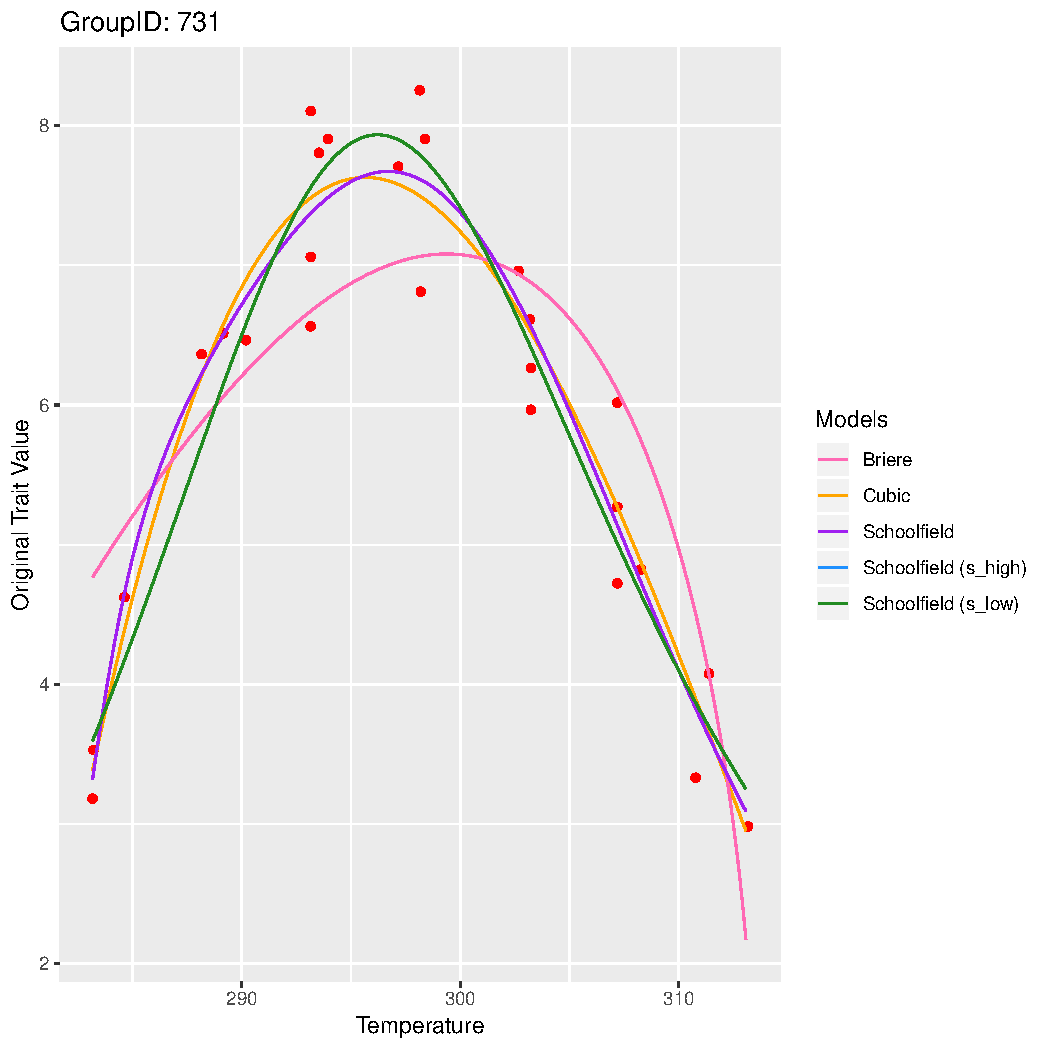
\includegraphics[width=\textwidth]{example4.pdf}
\end{figure}
Figure.4.GroupID 731
\\
\begin{figure}[H]
\centering
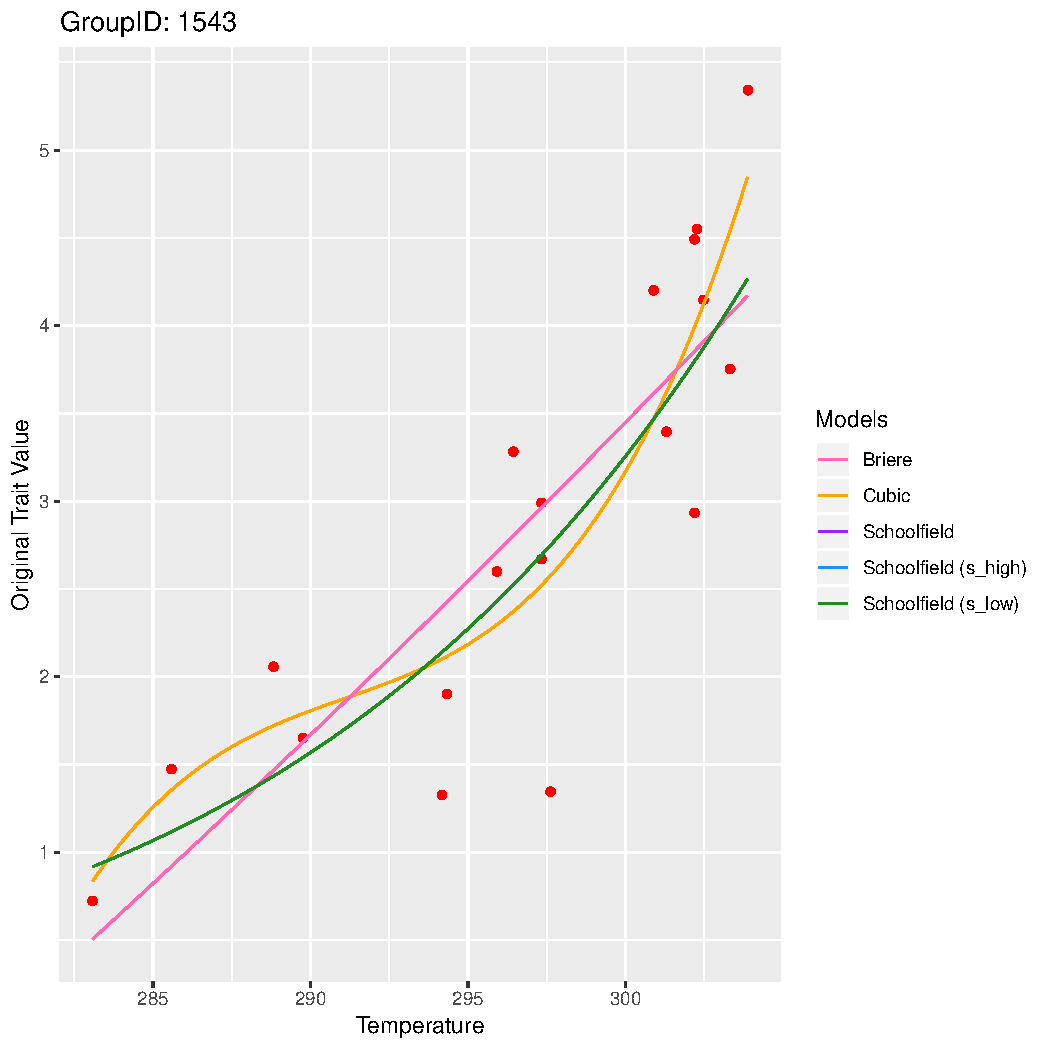
\includegraphics[width=\textwidth]{example5.pdf}
\end{figure}
Figure.5.GroupID 1543
\\
\\
The cubic model fitted in this dataset often exist in a single bell shape and some times a hyperbolic curve. The bell shape might not be completed in some cases as the observed data points are linear in distribution and forming half of the bell shape curve.
\\
The Briere model plots a straight line to predict the thermal response of metabolic rates. It can be a positive slope or negative depending on the data group.
\\
All of the 3 Schoolfield models plot a bell shape curve in either a completed way or one slope of the curve. In cases where both full and simplified Schoolfield models converge, they often have smiler curves. When both 2 simplified versions converge, these always show identical curves.
\subsection{Model comparison}
The AIC values obtained from 5 models in 1935 groups of data were all plot to the following figure. The x axis is group ID ranging from 1 to 1935 and y axis is the AIC value. Different colours were used to distinguish the 5 models. This figure directly displays the distribution of AIC and reflect the convergence status among 5 models and their relative fitness compared to others. 
\begin{figure}[H]
\centering
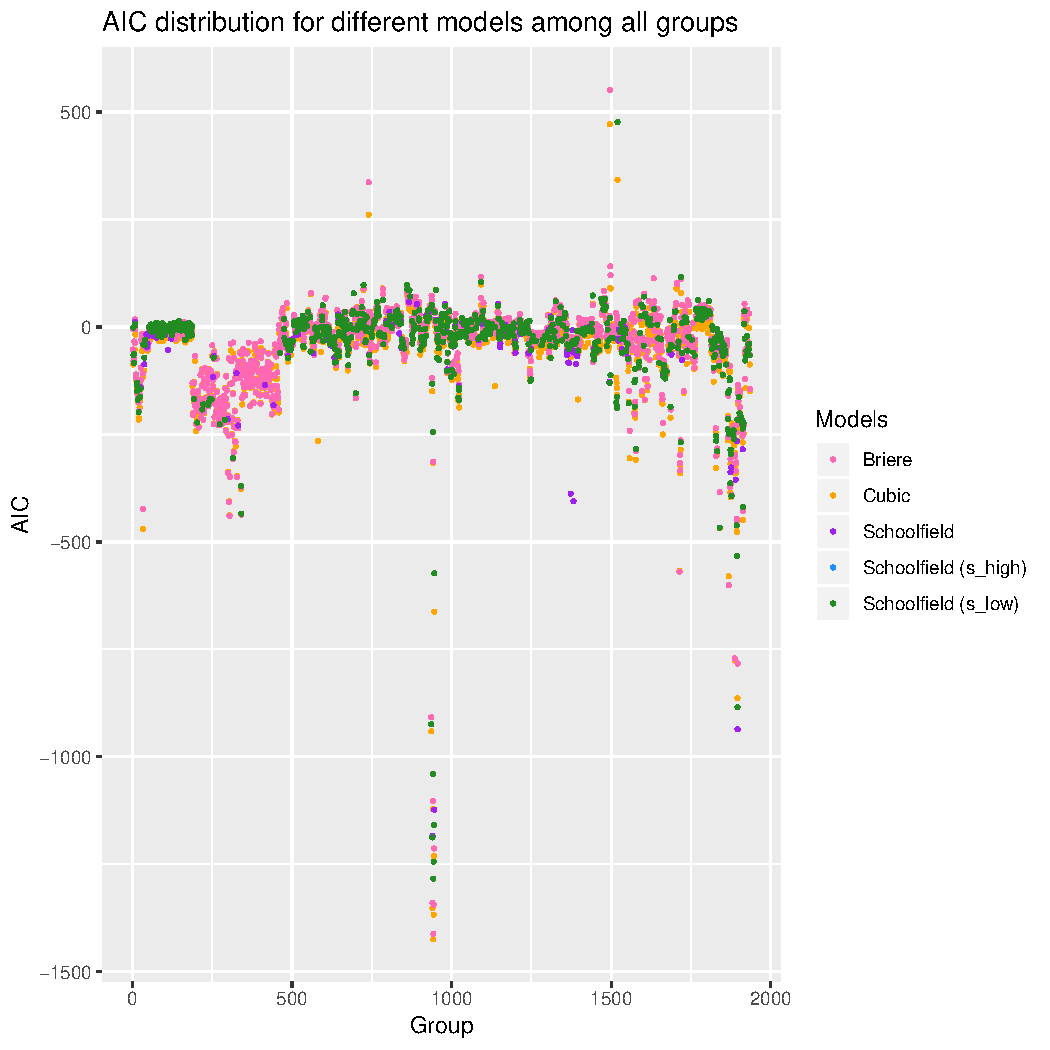
\includegraphics[width=\textwidth]{scatter_AIC.pdf}
\end{figure}
Figure.5.AIC distribution for different models among all groups
\\
\\
Meanwhile, the minimal AIC values among 5 models are selected in each case and the distribution is plotted in another figure. 
\begin{figure}[H]
\centering
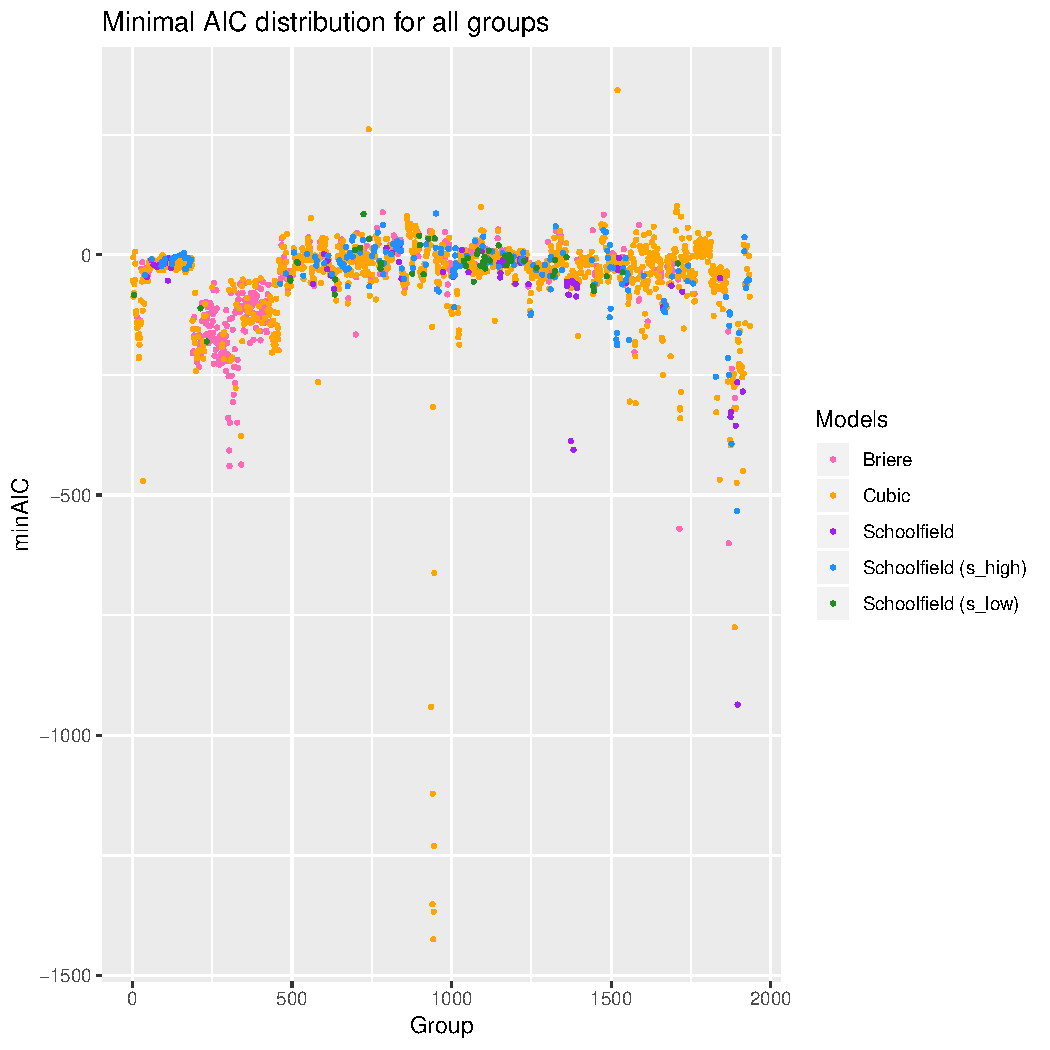
\includegraphics[width=\textwidth]{model_AIC.pdf}
\end{figure}
Figure.6.Minimal AIC distribution for all groups
\\
\\
The x axis is also group ID and y axis is the minimal AIC value among all converged models in the groups. Different colors is used to annotate different models. The minimal AIC values among the whole dataset ranges from -1424 to 342. For all 1935 groups of successful convergence, cubic model obtains the minimal AIC in 1204 groups, the ratio is about 0.62. For Briere model, it gets minimal AIC in 434 groups, comparing to 1913 groups it converges the ratio is about 0.23. The full Schoolfield model get 67 minimal AIC in 170 successfully converged groups, the ratio is about 0.40. The simplified version of Schoolfield model which focus on high temperature activities obtains 178 minimal AIC among 840 fitted models, the ratio is around 0.21. The other simplified Schoolfield model which ignores the high temperature effects has 52 minimal AIC values comparing to 530 groups of converged models, the ratio is close to 0.10.


\section{Discussion}
In general all 5 models are feasible models that can be applied to describe the thermal responses of metabolic traits. They all agree to the data for a certain extent, but with different limitations and applicability. 
\\
For cubic model, it converges at all groups in this dataset and also has relatively small AIC values compared to other models (minimal AIC rate is about 0.6), which indicates a good model. However, the cubic model is a phenomenological model which has no theory basis behind, therefore less interpretation provided for the mechanism of pattern. 
\\
For Briere model, it is also feasible to model the thermal response relationship for the majority of cases. However the fitted line is a linear line that fail to capture the curve relationship indicated by most of the observation groups. Meanwhile It is also lack of mechanic interpretation and has a relatively low better model percentage (the min AIC rate is only 0.2).
\\
The full Schoolfield model converges at the fewest data groups among 5 models. This result is expected, as it is the most complicated model. However the min AIC rate is around 0.4, which is the second better rate after cubic model. Also 352 groups failed to be modelled because the entries of data in these groups are fewer than the parameter number, which is not the case for other models and means that the full model should perform even better.
\\
When comparing the 2 simplified versions of Schoolfield model, the one focusing on high temperature behaviour (ignoring the low temperature inactivation rate) converge at more groups. This might suggest that in our study, the low temperature inactivation is relatively weak. Meanwhile, when both 2 simplified Schoolfield models converged, their fitted models are identical. This is also expected since these models are actually same except from initial parameters.
Although the simplified version converged in more groups, the AIC indicate that if the full model converge, the full model should be a better model to choose.
\\
In general, my personal opinion for modelling thermal response of metabolic trait is that: both cubic model and the full Schoolfield model are better models. The cubic model can be more universal to different groups of data when the theory basis of the model is not especially looked for. The full Schoolfield model is a good candidate if the mechanism behind the model is valued particularly.
\\
The are many limitation and more aspects to analyse in this study. The initial parameter estimation can be critical for the modelling result. If the initial parameter is given out of the scope of the tire parameters, the model might fail to converge. In this study, some initial parameters in some data groups for the 3 Schoolfield models failed to be estimated, as the distribution of datasets in those groups contain less information for the parameters to be calculated. And these end up in NA values which are allocated with median values based on other groups’ performance.
Moreover, the model selection process based on AIC is relatively instinctive. more quantified measurement should be made to compare the performance of models (based on AIC or not).
At last, the model performance among different types of original trait value is another potentially useful aspect to be analysed in the future.

\newpage


\bibliographystyle{plain}
\bibliography{miniproject}
\end{document}